\section{The VAMPIRES Instrument}\label{sec:design}

\begin{figure*}[t]
    \centering
    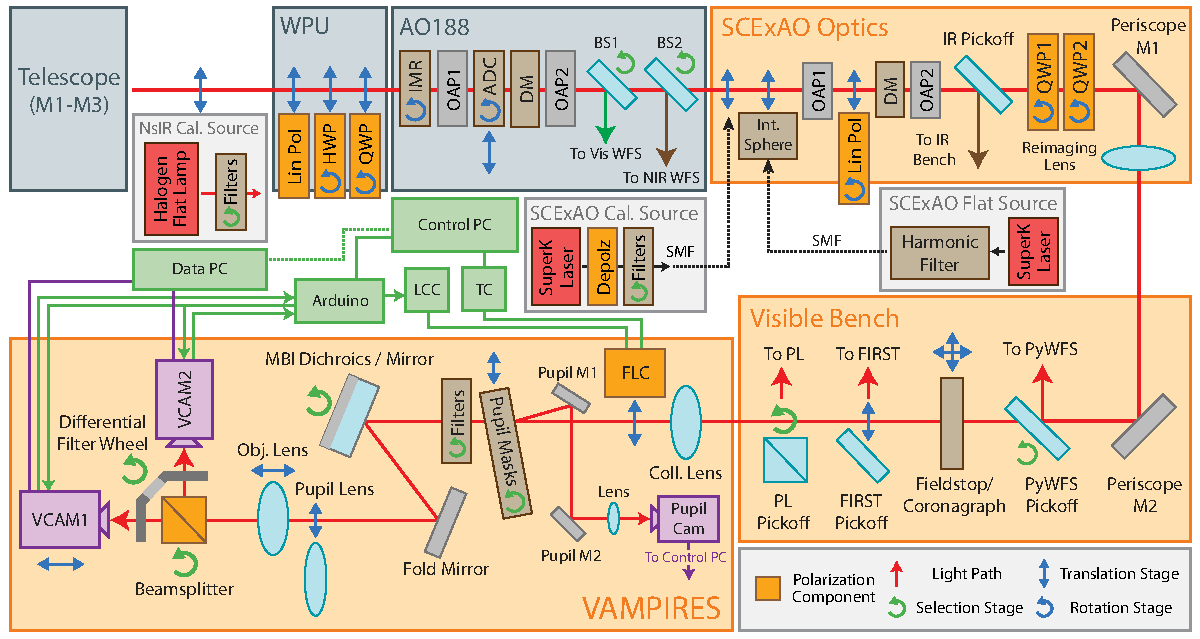
\includegraphics[width=\textwidth]{figures/VAMPIRES_diagram.pdf}
    \caption{VAMPIRES Instrument Schematic}
    \label{fig:schematic}
\end{figure*}

The Visible Aperture-Masking Polarimetric Imager/Interferometer for Resolving Exoplanetary Signatures (VAMPIRES) is the visible-light imager sub-instrument of the Subaru Coronagraphic Extreme Adaptive Optics testbed (SCExAO; \citet{jovanovic_subaru_2015}). SCExAO is a one-of-a-kind platform for high-contrast technological development and observations on the \SI{8.2}{\meter} Subaru telescope. SCExAO is mounted on the infrared Nasymth platform of Subaru behind the facility adaptive optics instrument, AO188 \citep{minowa_performance_2010}, which provides low-order correction with a curvature wavefront sensor to multiple instruments which are craned in and out of focus. AO188 also houses the K-mirror image rotator and atmospheric dispersion correcter (ADC).

The light from AO188 is split with a dichroic beamsplitter which transmits red to infrared light ($\lambda >$\SI{600}{\nano\meter}). This light enters SCExAO and is immediately collimated and corrected with a 2000-actuator Boston Micro Machines deformable mirror (DM), which has 45 actuators across the SCExAO pupil and operates at $\sim$\si{\kilo\hertz} speeds for extreme AO correction. Following the DM is a pupil mask which slightly undersizes the pupil (95\%, equivalent diameter of \SI{7.8}{\meter}) and blocks out two of the broken DM actuators. The beam is split with a near-IR dichroic filter ($\lambda=$\SI{950}{\nano\meter}), reflecting the visible light into a periscope which routes the beam onto a different optical bench and focuses the light with a reimaging lens.

Once the light is on the visible bench of SCExAO it encounters a series of pickoffs for routing the light to various modules of SCExAO. The first is the pickoff for the visible pyramid wavefront sensor (PyWFS), which has multiple filters for sending more or less light to the wavefront sensor to assure sufficient S/N during observations. Typically an \SI{800}{\nano\meter} dichroic filter is used, which effectively cuts off light below $\lambda <$\SI{775}{\nano\meter} due to its \ang{20} tilt. Then the light passes through a fieldstop that houses the suite of Lyot coronagraph masks (\autoref{sec:coronagraphy}) as well as a \SI{3}{\arcsecond}x\SI{3}{\arcsecond} fieldstop. After the fieldstop are two pickoffs for the fiber-fed instrument FIRST. These pickoffs typically use non-polarizing gray beamsplitters which allows simultaneous observations in VAMPIRES with appropriate focus shifts.

Finally, the remaining light (\SIrange{600}{775}{\nano\meter}) reaches the VAMPIRES collimating lens, after which is a deployable ferroelectric liquid crystal (FLC), a wheel for pupil-plane optics, and a standard filter wheel. The pupil wheel houses sparse aperture masks, neutral-density (ND) filters, and the coronagraph Lyot stops. This wheel is at $\sim$\ang{6} so that light reflected off the masks can be imaged by a separate pupil-viewing camera. The standard filter wheel houses five \SI{50}{\nano\meter}-wide bandpass filters for standard imaging as well as an empty slot for broadband observations, After this filter wheel is a separate baffle for the VAMPIRES fore-optics to reduce scattered light from motor encoders and electronic devices on the SCExAO bench. 

The beam then reaches a newly-developed multiband imaging (MBI) optic. This optic uses multiple dichroics with unique angles-of-incidence (AOI) to split broadband light into multiple fields imaged on the detector (\autoref{fig:mbi_schematic}). Our design uses three shortpass dichroic filters with a protected silver mirror at the back creating four $\sim$\SI{50}{\nano\meter} fields which roughly match the standard bandpass filters. This optic can be rotated \ang{180} to place a protected silver mirror in the beam, instead, creating a single image. In both cases, the light has a $\sim$\ang{10} reflection off a protected silver fold mirror before reaching the removable pupil-imaging lens and the objective lens.

\begin{figure}
    \centering
    \includegraphics[width=\columnwidth{figures/mbi_schematic.pdf}
    \caption{Schematic drawing for the multiband imaging dichroic principle. Broadband collimated light reaches the stack of dichroics plus mirror, each of which has a unique angle of incidence (AOI). The light reflected by each dichroic will have its own field in the focal plane due to the AOI. The light transmitted by each dichroic will pass onto the next optic, until all remaining light is reflected by a mirror at the back. of the stack.\label{fig:mbi_schematic}}
    
\end{figure}

As the light is focusing it passes through the beamsplitter wheel, which has a non-polarizing 50/50 beamsplitter cube, a wire-grid polarizing beamsplitter cube, or the light can be imaged without a beamsplitter onto a single detector, only. Because the beamsplitter cubes are \SI{25}{\milli\meter} thick, there is a significant focus shift which is accomadated by a translation stage on one of the cameras and the objective lens. The last optic before the detectors is a differential filter wheel which houses four narrowband filters. These filters come in pairs and are deployed so each pair is imaged simultaneously in front of both cameras. The filter wheel can switch which camera a respective filter is in front of with a \ang{180} rotation, which allows differential imaging to cancel out the non-common path aberrations between the two beams \citep{uyama_high-contrast_2020}.

\begin{deluxetable}{cl}
\tabletypesize{\footnotesize}
\tablehead{
    \colhead{Name} & 
    \colhead{Value(s)}
}
\tablecaption{VAMPIRES specifications.\label{tbl:specs}}
\startdata
Diff. Limit & \SI{16.5}{\mas} at \SI{625}{\nm}, \SI{20.1}{\mas} at \SI{760}{\nm}\\
FOV & \SI{3}{\arcsecond} x \SI{3}{\arcsecond} \\
Plate Scale & \SI{6.01}{\mas} \\
Inst. PA & \ang{-41.4} \\
Coronagraph & CLC-2, CLC-3, CLC-5, CLC-7, DGVVC \\
SAM & 7-hole, 9-hole, 18-hole, Annulus \\
Pupil Masks & LyotStop, RAP, Mirror, ND1.0, ND2.5 \\
Filters & 625-50, 650-50, 675-50, 725-50, 750-50, 775-50, \\
& Open, MBI \\
NB Filters & H$\alpha$, H$\alpha$-Cont, SII, SII-Cont \\
Beamsplitter & PBS, NPBS, Open \\
Polarimetry & HWP + PBS, HWP + FLC + PBS \\
\enddata
\end{deluxetable}
